\documentclass[11pt]{article}

% Language setting
\usepackage[turkish]{babel}
\usepackage{pythonhighlight}

\usepackage[a4paper,top=2cm,bottom=2cm,left=2cm,right=2cm,marginparwidth=2cm]{geometry}

% Useful packages
\usepackage{amsmath}
\usepackage{graphicx}
\usepackage[colorlinks=true, allcolors=blue]{hyperref}
\usepackage{verbatim}
\usepackage{fancyhdr} % for header and footer
\usepackage{titlesec}
\usepackage{parskip}

\setlength{\parindent}{0pt}

\titleformat{\subsection}[runin]{\bfseries}{\thesubsection}{1em}{}

\pagestyle{fancy} % activate the custom header/footer

% define the header/footer contents
\lhead{\small{23BLM-4014 Yapay Sinir Ağları Ara Sınav Soru ve Cevap Kağıdı}}
\rhead{\small{Dr. Ulya Bayram}}
\lfoot{}
\rfoot{}

% remove header/footer on first page
\fancypagestyle{firstpage}{
  \lhead{}
  \rhead{}
  \lfoot{}
  \rfoot{\thepage}
}
 

\title{Çanakkale Onsekiz Mart Üniversitesi, Mühendislik Fakültesi, Bilgisayar Mühendisliği Akademik Dönem 2022-2023\\
Ders: BLM-4014 Yapay Sinir Ağları/Bahar Dönemi\\ 
ARA SINAV SORU VE CEVAP KAĞIDI\\
Dersi Veren Öğretim Elemanı: Dr. Öğretim Üyesi Ulya Bayram}
\author{%
\begin{minipage}{\textwidth}
\raggedright
Öğrenci Adı Soyadı: Bora Yörümüş\\ % Adınızı soyadınızı ve öğrenci numaranızı noktaların yerine yazın
Öğrenci No: 190401041
\end{minipage}%
}

\date{14 Nisan 2023}

\begin{document}
\maketitle

\vspace{-.5in}
\section*{Açıklamalar:}
\begin{itemize}
    \item Vizeyi çözüp, üzerinde aynı sorular, sizin cevaplar ve sonuçlar olan versiyonunu bu formatta PDF olarak, Teams üzerinden açtığım assignment kısmına yüklemeniz gerekiyor. Bu bahsi geçen PDF'i oluşturmak için LaTeX kullandıysanız, tex dosyasının da yer aldığı Github linkini de ödevin en başına (aşağı url olarak) eklerseniz bonus 5 Puan! (Tavsiye: Overleaf)
    \item Çözümlerde ya da çözümlerin kontrolünü yapmada internetten faydalanmak, ChatGPT gibi servisleri kullanmak serbest. Fakat, herkesin çözümü kendi emeğinden oluşmak zorunda. Çözümlerinizi, cevaplarınızı aşağıda belirttiğim tarih ve saate kadar kimseyle paylaşmayınız. 
    \item Kopyayı önlemek için Github repository'lerinizin hiçbirini \textbf{14 Nisan 2023, saat 15:00'a kadar halka açık (public) yapmayınız!} (Assignment son yükleme saati 13:00 ama internet bağlantısı sorunları olabilir diye en fazla ekstra 2 saat daha vaktiniz var. \textbf{Fakat 13:00 - 15:00 arası yüklemelerden -5 puan!}
    \item Ek puan almak için sağlayacağınız tüm Github repository'lerini \textbf{en geç 15 Nisan 2023 15:00'da halka açık (public) yapmış olun linklerden puan alabilmek için!}
    \item \textbf{14 Nisan 2023, saat 15:00'dan sonra gönderilen vizeler değerlendirilmeye alınmayacak, vize notu olarak 0 (sıfır) verilecektir!} Son anda internet bağlantısı gibi sebeplerden sıfır almayı önlemek için assignment kısmından ara ara çözümlerinizi yükleyebilirsiniz yedekleme için. Verilen son tarih/saatte (14 Nisan 2023, saat 15:00) sistemdeki en son yüklü PDF geçerli olacak.
    \item Çözümlerin ve kodların size ait ve özgün olup olmadığını kontrol eden bir algoritma kullanılacaktır. Kopya çektiği belirlenen vizeler otomatikman 0 (sıfır) alacaktır. Bu nedenle çözümlerinizi ve kodlarınızı yukarıda sağladığım gün ve saatlere kadar kimseyle paylaşmayınız.
    \item Bu vizeden alınabilecek en yüksek not 100'dür. Toplam aldığınız puan 100'ü geçerse, aldığınız not 100'e sabitlenecektir.
    \item LaTeX kullanarak PDF oluşturanlar öz geçmişlerine LaTeX bildiklerini de eklemeyi unutmasınlar :)
    \item Bu vizedeki soruların çözümleri ve tex dosyası için istediğiniz kadar sayıda Github repository'si oluşturabilirsiniz. Sadece yukarıda belirttiğim tarihlerde (14 Nisan 2023 saat 15:00 ile 15 Nisan 2023 saat 15:00 arasında) public yapmayı/halka açmayı ve Github profilinizi de öz geçmişinize eklemeyi unutmayın :)
    \item Bilgisayarınıza hiçbir program kurmadan, Overleaf, Google Colab, Kaggle gibi ortamlar üzerinden bu vizeyi tamamlamanız mümkün. İyi çalışmalar!!
\end{itemize}

(Ekstra 5 puan) \url{https://github.com/yorumusb/Yapay-Sinir-Aglari}

\newpage
\section{(Toplam 10 Puan) Hopfield Networks:}

\subsection{(2 Puan)} \textbf{ChatGPT’ye size Hopfield Network’ler ile ilgili detaylı bilgi vermesini isteyin. Sorduğunuz soruyu, ChatGPT'nin çıkartığı cevabı aşağı koyun. Bu cevapta anlamadığınız terimleri de ChatGPT’ye sorup, sorduğunuz soruları ve ChatGPT’nin verdiği cevapları da sırayla aşağı koyun.}

\textbf{Soru: Hopfield Network’ler ile ilgili detaylı bilgi verir misin}


Elbette, Hopfield ağları, yapay sinir ağları sınıfına ait bir türdür ve adını John Hopfield'den almıştır. Hopfield ağları, bir dizi nöronun birbirine bağlanmasıyla oluşan bir ağdır ve genellikle öğrenme ve hatırlama işlemleri için kullanılır.

Hopfield ağları, aslında bir tür geri beslemeli ağdır ve her bir nöron, diğer nöronlardan aldığı girdilere dayanarak kendi çıktısını hesaplar. Hopfield ağlarında her bir nöron iki durumda olabilir: 1 veya -1. Bu nöronların çıktıları, belirli bir enerji fonksiyonu kullanılarak hesaplanır.

Öğrenme sürecinde, Hopfield ağı, bir dizi örnek veri kümesi ile eğitilir. Bu örnekler ağın belleğinde depolanır ve daha sonra hatırlama işleminde kullanılır. Hatırlama işlemi, ağa verilen kısmi veya bozuk bir girdiye dayanarak, ağın belleğindeki en yakın örneği hatırlamasını gerektirir.

Hopfield ağlarının bir diğer önemli özelliği de, enerji fonksiyonu kullanarak bir enerji yüzeyi oluşturmalarıdır. Bu enerji yüzeyi, ağın durumuna ve belleğindeki verilere bağlıdır ve ağın enerji düzeyini tanımlar. Enerji yüzeyindeki minimum noktalar, ağın belleğinde depolanan örnek verileri temsil eder.

Hopfield ağları, özellikle desen tanıma, veri sıkıştırma ve optimizasyon problemleri için kullanılır. Ayrıca, Hopfield ağları hala yapay zeka araştırmalarında aktif bir alandır ve daha gelişmiş tekniklerle birlikte kullanıldıklarında daha da etkili hale gelebilirler.

\textbf{Soru: Hopfield sinir ağları neden bilinmelidir}

Hopfield sinir ağları, yapay sinir ağları alanında oldukça önemli bir rol oynar ve çeşitli uygulamalarda kullanılır. İşte Hopfield sinir ağlarının neden bilinmesi gerektiği ile ilgili birkaç neden:

Asosyal hafıza işlevi: Hopfield sinir ağları, hafızaya dayalı birçok problemi çözmek için kullanılabilir. Bu sinir ağları, özellikle asosyal hafıza işlevi gösterir, yani belirli bir bilgi seti ile öğrenilir ve daha sonra bu bilgileri hatırlamak için kullanılabilir.

Patern tanıma: Hopfield sinir ağları, desen tanıma problemlerini çözmek için kullanılabilir. Örneğin, bir Hopfield sinir ağı, bir görüntünün yeniden yapılandırılmasını gerçekleştirebilir.

Optimizasyon: Hopfield sinir ağları, optimizasyon problemlerini çözmek için de kullanılabilir. Örneğin, bir Hopfield sinir ağı, bir enerji fonksiyonunu minimize ederek en iyi çözümü bulabilir.

Paralel işleme: Hopfield sinir ağları, paralel işleme özellikleri sayesinde hızlı bir şekilde büyük veri kümelerini işleyebilirler.

Hopfield sinir ağları, bu özellikleri nedeniyle birçok alanda kullanılmaktadır ve yapay sinir ağları alanındaki temel konulardan biridir. Bu nedenle, yapay zeka ve makine öğrenmesi alanında çalışanlar Hopfield sinir ağları hakkında bilgi sahibi olmalıdır.

\textbf{Soru: geri beslemeli ağ ne demek}

Geri beslemeli ağ, bir nöronun çıktısı, aynı ağda başka bir nörona veya kendisine geri gönderildiğinde oluşan ağdır. Bu geri bildirim, bir önceki adımda oluşan çıktıyı, sonraki adımlarda girdi olarak kullanmasına izin verir. Bu nedenle, geri beslemeli ağlar, girdi sinyalleri ile birlikte önceki çıktıların da ağda dolaştığı bir döngüsel yapıya sahiptirler.

Geri beslemeli ağlar, genellikle dinamik sistemleri modellemek, hatırlama işlemlerini gerçekleştirmek ve çeşitli işlemlerde girdi sinyallerini düzenlemek için kullanılır. Bu ağlar, örneğin, zaman serilerindeki trendleri ve döngüleri tespit etmek, sinyal işleme uygulamalarında gürültüyü filtrelemek ve hatta insan davranışını modellemek için kullanılabilir.

Geri beslemeli ağların bir diğer önemli özelliği, ağın belleğinde geçmiş durumların depolanabilmesidir. Bu bellek, ağın önceki adımlarında aldığı kararları ve çıktıları hatırlamasına izin verir ve bu nedenle geri beslemeli ağlar, özellikle zamana bağlı verilerin işlenmesi ve tahmini için yararlıdır.

\textbf{Soru: Bahsedilen enerji fonksiyonu nedir}

Enerji fonksiyonları, bir sistemdeki durumların belirli özelliklerini tanımlayarak farklı durumların sistemdeki davranışını etkileyebilir.
Bir yapay sinir ağı için enerji fonksiyonu, ağın belleğindeki depolanan örneklerin benzerliklerine dayanarak hatırlama işlemini gerçekleştirebilir. Enerji fonksiyonları, sistem davranışını analiz etmek ve optimize etmek için de kullanılabilir.

\textbf{Soru: yapay sinir ağlarında enerji yüzeyi ne demektir}

Yapay sinir ağları, makine öğrenmesi algoritmalarıdır ve öğrenme sürecinde genellikle bir hata fonksiyonu kullanılır. Enerji yüzeyi, bu hata fonksiyonunun bir gösterimidir ve yapay sinir ağlarının optimize edilmesinde kullanılır.

\subsection{(8 Puan)} \textbf{ChatGPT’nin açıklamalarından ne anladığınızı buraya kendi kelimelerinizle özetleyin. Örneğin ``Hopfield Network nedir? Ne işe yarar? Neden bilmemiz gerekir bunu? Gerçek hayatta kullanılıyor mu?'' gibi. Anlamadığınız kısımlar varsa ve ChatGPT’nin açıklamaları yeterli gelmezse internet dahil farklı kaynaklardan araştırıp, bilgilerin doğruluğunu sorgulamakta serbestsiniz. Konuyu doğru anlayıp anlamamanız puana etki edecektir. Kullandığınız kaynakları da belirtin!}

Hopfield sinir ağları'nın, geri beslemeli bir yapay sinir ağı türü olduğunu,
Nöronların bağlantısıyla oluştuğunu,
Asosyal hafıza işlevi, patern tanıma, optimizasyon, paralel işleme gibi özelliklere sahip olduğunu ve yapay sinir ağlarının temellerinden olduğunu, Gerçek hayatta özellikle bellek ve optimizasyon problemlerinin çözümünde kullanıldığını öğrendim. Bu bilgilere ChatGPT ve

https://en.wikipedia.org/wiki/Hopfield\_network 

üzerinden ulaştım


\section{(Toplam 10 Puan) Boltzman Machine:}

\subsection{(2 Puan)} \textbf{ChatGPT’ye size Boltzman Machine ilgili detaylı bilgi vermesini isteyin. Sorduğunuz soruyu, ChatGPT'nin çıkartığı cevabı aşağı koyun. Bu cevapta anlamadığınız terimleri de ChatGPT’ye sorup, sorduğunuz soruları ve ChatGPT’nin verdiği cevapları da sırayla aşağı koyun.}

\textbf{Soru: Boltzman Machine ile ilgili detaylı bilgi verir misin}

Boltzmann makinesi, bir tür yapay sinir ağıdır. İlk kez 1985 yılında Geoffrey Hinton ve Terry Sejnowski tarafından tanıtılmıştır. Adını fizikteki Boltzmann dağılımından almıştır. Boltzmann makinesi, özellikle sınıflandırma ve veri sıkıştırma gibi problemler için kullanılabilen bir çeşit yapay sinir ağıdır.

Bir Boltzmann makinesi, giriş verilerini alan ve bir çıktı üreten bir sistemdir. Ancak, Boltzmann makinesi aynı zamanda içinde bulunduğu ortamla etkileşim halindedir ve bu ortamın da bir etkisi vardır. Boltzmann makinesi, birbirine bağlı birçok nöron ağından oluşur. Bu nöronlar, birbirleriyle bağlantılıdır ve bu bağlantılar rastgele olarak belirlenir. Boltzmann makinesi, birçok nöronun bir arada çalışmasıyla verileri anlamak ve sınıflandırmak için kullanılır.

Bir Boltzmann makinesi, iki tür nöron içerir: görünür nöronlar ve gizli nöronlar. Görünür nöronlar, verilerin girdiği noktalardır. Gizli nöronlar, verilerin anlamını belirleyen nöronlardır. Bu iki tür nöron, birbirleriyle bağlantılıdır. Bağlantıların güçleri, bir ağırlık matrisi tarafından belirlenir.

Bir Boltzmann makinesi, enerji fonksiyonu olarak adlandırılan bir matematiksel fonksiyon kullanır. Bu fonksiyon, nöronların durumlarını (açık veya kapalı) kullanarak sistemin enerjisini hesaplar. Boltzmann makinesi, enerjiyi en aza indirmeye çalışarak işlev görür. Bu, bir optimizasyon problemi olarak düşünülebilir. Boltzmann makinesi, enerjinin minimum olduğu duruma ulaştığında, çıktısını verir.

Bir Boltzmann makinesi, çeşitli amaçlar için kullanılabilir. Örneğin, veri sıkıştırma problemleri için kullanılabilir. Bu durumda, Boltzmann makinesi, verileri küçük bir sayıda gizli nöron kullanarak temsil edebilir. Bu, daha az veri saklamak ve daha hızlı işlem yapmak için kullanılabilir. Boltzmann makinesi, ayrıca sınıflandırma problemleri için de kullanılabilir. Bu durumda, makine, verileri sınıflara ayırmak için kullanılabilir.

Boltzmann makinesi, daha büyük ve daha karmaşık yapay sinir ağları olan derin öğrenme modellerinin temelini oluşturur. Ancak, Boltzmann makinesi, son yıllında kullanımı biraz azalmıştır çünkü eğitimi oldukça zor ve zaman alıcıdır. Bununla birlikte, Boltzmann makineleri, özellikle sınıflandırma ve veri sıkıştırma problemlerinde iyi performans gösterirler. Ayrıca, çeşitli diğer uygulamalarda da kullanılabilirler, örneğin doğal dil işleme ve örüntü tanıma gibi alanlarda kullanılabilirler.

Boltzmann makinesi, eğitimi oldukça zor olan bir modeldir. Eğitim, Gibbs örneklemesi adı verilen bir yöntem kullanılarak gerçekleştirilir. Bu yöntem, sistemin olası durumlarını örnekleyerek modelin öğrenmesine yardımcı olur. Ancak, eğitim süreci oldukça yavaştır ve büyük veri kümeleri için uygun değildir. Bu nedenle, Boltzmann makinesi, derin öğrenme modellerinin daha gelişmiş varyasyonlarıyla değiştirilmiştir.

Sonuç olarak, Boltzmann makinesi, yapay sinir ağlarının öncüllerinden biridir. Veri sıkıştırma ve sınıflandırma gibi problemler için kullanılabilir. Ancak, eğitimi oldukça zor ve zaman alıcıdır. Bu nedenle, daha gelişmiş yapay sinir ağı modelleri, Boltzmann makinelerinin yerini almıştır.

\textbf{Soru: Boltzmann dağılımı nedir}

Boltzmann dağılımı, istatistiksel mekanikte bir sistemdeki parçacıkların enerji dağılımını tanımlayan bir olasılık dağılımıdır. Bu dağılım, parçacıkların enerji seviyelerinin olasılık dağılımını ifade eder.

Boltzmann dağılımı, bir sistemin sıcaklığı ve enerji durumu arasındaki ilişkiyi gösterir. Bu dağılım, bir sistemdeki parçacıkların enerji seviyelerinin olasılıklarını, sistemdeki toplam enerji seviyesine ve sıcaklığa bağlı olarak hesaplar.

Boltzmann dağılımı ayrıca, termodinamik dengede olan sistemlerin davranışını da açıklamaktadır. Termodinamik denge, sistemdeki enerjinin homojen olarak dağıldığı bir durumdur ve bu durumda Boltzmann dağılımı geçerlidir.

Boltzmann dağılımı, fizikte, kimyada ve mühendislikte kullanılan birçok modelleme ve hesaplama yönteminde kullanılır.

\textbf{Soru: Boltzmann da ortam nasıl etki eder}

Boltzmann dağılımı, bir sistemin sıcaklığına bağlı olarak parçacıkların enerji seviyelerinin olasılık dağılımını belirler. Bu nedenle, sistemdeki ortam sıcaklığı, Boltzmann dağılımı üzerinde önemli bir etkiye sahiptir.

Sıcaklık arttıkça, sistemin içindeki parçacıkların enerji seviyeleri yükselir ve daha fazla sayıda parçacık yüksek enerji seviyelerinde bulunur. Bu da Boltzmann dağılımındaki olasılık dağılımını değiştirir ve enerjisi yüksek olan durumların daha olası hale gelmesine neden olur.

Bunun yanı sıra, ortamın yoğunluğu da Boltzmann dağılımı üzerinde etkili olabilir. Yoğunluk arttıkça, parçacıkların birbirleriyle çarpışma olasılığı artar ve bu da enerji seviyeleri arasındaki dağılımı etkiler.

Sonuç olarak, Boltzmann dağılımı, sistemdeki ortamın sıcaklık ve yoğunluğu gibi faktörlere bağlı olarak değişir. Bu nedenle, bir sistemin davranışını anlamak ve öngörmek için, ortamın etkilerinin de göz önünde bulundurulması gereklidir.

\textbf{Soru: ağırlık matrisi nedir}

Boltzmann makinelerinde, girdi ve çıktı arasındaki ilişkileri öğrenmek için bir ağırlık matrisi kullanılır. Bu ağırlık matrisi, sistemin enerji fonksiyonunu tanımlayan bir matristir ve Boltzmann makinesindeki nöronların etkileşimlerini gösterir.

Boltzmann ağırlık matrisi, nöronların arasındaki bağlantıları gösteren bir matristir. Bu matris, iki katman arasındaki bağlantıları gösterir. Girdi katmanındaki nöronlar, ağırlık matrisindeki birinci boyutta, çıktı katmanındaki nöronlar ise ikinci boyutta temsil edilir.

Ağırlık matrisinin her bir öğesi, bir nöronun diğer nöronlarla olan bağlantısının gücünü temsil eder. Bu ağırlık matrisindeki değerler, ağın öğrenme sürecinde otomatik olarak belirlenir. Bu süreçte, ağırlık matrisindeki değerler, verilen girdiler ve beklenen çıktılar arasındaki farkları minimize etmek için ayarlanır.

Boltzmann ağırlık matrisi, ağın performansını ve öğrenme kapasitesini etkileyen önemli bir faktördür. Matrisin boyutu, katman sayısı, nöron sayısı ve ağın öğrenme hızı gibi faktörler, matrisin etkinliğini belirleyebilir.

\textbf{Soru: daha gelişmiş yapay sinir ağı modelleri nelerdir}

Yapay sinir ağları (YSA), son yıllarda büyük ilerleme kaydetmiş ve birçok alanda kullanılmaktadır. Geleneksel YSA'ların yanı sıra, daha gelişmiş YSA'lar da vardır. Bazı örnekleri aşağıda verilmiştir:

Derin Öğrenme: Derin öğrenme, çok katmanlı sinir ağları kullanarak verileri otomatik olarak öğrenme yöntemidir. Bu yöntem, özellikle görüntü, ses ve doğal dil işleme alanlarında başarılı sonuçlar vermektedir.

Rekürsif Yapay Sinir Ağları: Rekürsif Yapay Sinir Ağları (RNN'ler), zaman serileri ve sıralı veriler gibi zaman bağımlı verileri işlemek için kullanılır. Bu ağlar, önceki adımlarda hesaplanan çıktıları yeni girdilere dahil eder.

Evrişimli Sinir Ağları: Evrişimli Sinir Ağları (CNN'ler), görüntü işleme ve ses işleme gibi uygulamalar için tasarlanmıştır. Bu ağlar, verilerdeki özellikleri tanımlamak ve sınıflandırmak için evrişim filtreleri kullanır.

Otomatik Kodlayıcılar: Otomatik Kodlayıcılar, verileri daha az boyutta temsil etmek için kullanılır. Bu ağlar, verilerin özelliklerini otomatik olarak öğrenir ve daha sonra bu özellikleri kullanarak verileri daha küçük boyutta temsil eder.

Rekabetçi Yapay Sinir Ağları: Rekabetçi Yapay Sinir Ağları, öğrenme sürecinde rekabetçi bir ortam kullanır. Bu ağlar, verileri kümelemek ve sınıflandırmak için kullanılır.

Bu gelişmiş YSA'lar, farklı veri türleri ve uygulamalar için özelleştirilmiştir. Bu nedenle, doğru yöntemin seçilmesi, verilerin ve uygulamanın gereksinimlerine bağlıdır.

\subsection{(8 Puan)} \textbf{ChatGPT’nin açıklamalarından ne anladığınızı buraya kendi kelimelerinizle özetleyin. Örneğin ``Boltzman Machine nedir? Ne işe yarar? Neden bilmemiz gerekir bunu? Gerçek hayatta kullanılıyor mu?'' gibi. Anlamadığınız kısımlar varsa ve ChatGPT’nin açıklamaları yeterli gelmezse internet dahil farklı kaynaklardan araştırıp, bilgilerin doğruluğunu sorgulamakta serbestsiniz. Konuyu doğru anlayıp anlamamanız puana etki edecektir. Kullandığınız kaynakları da belirtin!}

Boltzman Machine'in bir yapay sinir ağı olduğunu sınıflandırma ve sıkıştırma gibi problemler için kullanıldığını, bulunduğu ortamla etkileşim içinde olduğunu ve bu ortamda rastgele şekilde birbirine bağlanan nöronların ortak çalışmasıyla girdi ve çıktılar ürettiğini, nöronların durumlarıyla sistemin enerjisini hesapladığını ve bu enerjinin en aza indiği durumda çıktı vereceğini, derin öğrenme modelinin bir temeli olduğunu ancak zor ve zaman alıcı bir öğrenme süreci olduğu için kullanımının azaldığını ve derin öğrenmenin daha gelişmiş versiyonlarının Boltzman'ın yerini aldığını öğrendim. Kaynak olarak ChatGPT ve
https://en.wikipedia.org/wiki/Boltzmann\_machine
kullandım

\section{(Toplam 10 Puan) Markov Assumption ve Markov Chain:}

\subsection{(2 Puan)} \textbf{ChatGPT’ye size Markov assumption ve Markov Chain ilgili detaylı bilgi vermesini isteyin. Sorduğunuz soruyu, ChatGPT'nin çıkartığı cevabı aşağı koyun. Bu cevapta anlamadığınız terimleri de ChatGPT’ye sorup, sorduğunuz soruları ve ChatGPT’nin verdiği cevapları da sırayla aşağı koyun.}

\textbf{Soru: Markov assumption ve Markov Chain ile ilgili detaylı bilgi verir misin}

Markov karar süreci, belirli bir sistemi tanımlayan ve bir ajanın bu sistemi etkileme sürecini modelleyen bir matematiksel çerçevedir. Markov karar süreci, bir sonraki durumun sadece mevcut durumunun bir fonksiyonu olduğu Markov zinciri varsayımına dayanmaktadır.

Markov zinciri, belirli bir sistemi tanımlayan bir olasılık sürecidir. Bu süreçte, gelecekteki durumlar, yalnızca mevcut durumun bir fonksiyonu ve geçmiş durumların değerleriyle ilgili olmayan bir rastgele değişkene bağlıdır. Bu nedenle, Markov zinciri, geçmiş durumların ve gelecekteki durumların bağımsız olduğunu varsayar.

Markov zinciri, bir dizi durumdan oluşur ve her durum, bir sonraki duruma geçiş olasılıklarının belirlenmesi için bir durum uzayı tarafından tanımlanır. Bu geçiş olasılıkları, durumların geçiş matrisi olarak adlandırılan bir matris tarafından temsil edilir. Bu matris, her bir satırı mevcut durumun, her bir sütunu da bir sonraki durumun olasılıklarını içerir.

Markov zinciri, çeşitli uygulamalarda kullanılmaktadır. Örneğin, finansal piyasalarda, gelecekteki fiyat hareketlerini modellemek için kullanılır. Ayrıca, makine öğrenmesinde, doğal dil işlemede, işletme yönetiminde ve diğer birçok alanda kullanılır.

\textbf{Soru: Markov assumption ve Markov Chain ne işe yarar}

Markov varsayımı ve Markov zinciri, birçok farklı uygulama alanında kullanılan matematiksel araçlardır.

Markov varsayımı, bir sistemi tanımlayan bir modelde, bir sonraki durumun yalnızca mevcut durumun bir fonksiyonu olduğunu varsayar. Bu varsayım, sistemin gelecekteki durumunu tahmin etmek için gereken bilgiyi en aza indirir ve modelin hesaplama yükünü azaltır. Bu nedenle, birçok uygulamada, Markov varsayımı kullanarak modelin hesaplama maliyetini azaltmak mümkündür.

Markov zinciri ise, belirli bir sistemi tanımlayan ve bir sonraki durumun yalnızca mevcut durumun bir fonksiyonu olduğu bir olasılık sürecidir. Markov zinciri, çeşitli uygulamalarda kullanılır, özellikle de rastgele süreçlerin modellemesi ve analizi için. Örneğin, finansal piyasalarda, gelecekteki fiyat hareketlerini modellemek için Markov zinciri kullanılabilir. Ayrıca, doğal dil işlemede, makine öğrenmesinde ve işletme yönetiminde de kullanılır.

Markov zinciri, gelecekteki durumların yalnızca mevcut durumun bir fonksiyonu olduğu varsayımıyla çalışır. Bu nedenle, birçok uygulamada, Markov zinciri, gelecekteki durumların tahmin edilmesi veya bir sistemdeki davranışların analiz edilmesi için kullanılır. Örneğin, bir araba navigasyon sistemini düşünelim. Arabanın mevcut konumu, hızı, yönü ve diğer faktörler, Markov zincirinin mevcut durumunu oluşturur. Bu durumda, arabanın bir sonraki konumu, hızı ve yönü, mevcut durumun bir fonksiyonu olarak tahmin edilebilir.

Özetle, Markov varsayımı ve Markov zinciri, birçok uygulamada, özellikle rastgele süreçlerin modellemesi ve analizi için kullanılan matematiksel araçlardır.

\textbf{Soru: Markov assumption ve Markov Chain nasıl kullanılır}

Markov varsayımı ve Markov zinciri, birçok farklı alanda kullanılabilir. İşte bu araçların bazı kullanımları:

Doğal Dil İşlemede: Markov zinciri, doğal dil işleme uygulamalarında sıklıkla kullanılır. Örneğin, bir cümledeki kelimelerin sıralaması, bir Markov zinciri olarak modellenebilir. Bu modele dayalı olarak, bir sonraki kelimenin ne olabileceği tahmin edilebilir.

Finansal Analizde: Markov zinciri, finansal analizde kullanılan birçok modelde kullanılabilir. Örneğin, bir hisse senedinin fiyat hareketlerini tahmin etmek için Markov zinciri kullanılabilir. Bu, geçmiş fiyat hareketlerine dayalı olarak, gelecekteki fiyat hareketlerinin belirli bir olasılık dağılımına göre tahmin edilmesini sağlar.

Robotikte: Markov zinciri, robotikte çevre bilgisinin işlenmesi ve robotun hareketlerinin kontrolü için kullanılabilir. Örneğin, bir robotun hareketlerinin sonraki adımını belirlemek için, mevcut durumu ve önceden tanımlanmış hareket seçeneklerini bir Markov zincirinde modelleyebilirsiniz.

Makine Öğrenmesinde: Markov zinciri, makine öğrenmesi algoritmalarında da kullanılabilir. Örneğin, bir müşterinin alışveriş davranışları Markov zinciriyle modelleyebilir ve bu modele dayalı olarak, müşterinin gelecekte hangi ürünleri satın alabileceği tahmin edilebilir.

Markov varsayımı ve zinciri, herhangi bir sistemi modellerken, sistemin mevcut durumuna ve olasılık dağılımına dayalı olarak gelecekteki durumları tahmin etmek için kullanılabilir. Bu araçlar, özellikle rastgele süreçlerin modellemesi ve analizi için kullanışlıdır ve birçok farklı uygulama alanında yaygın olarak kullanılırlar.

\subsection{(8 Puan)} \textbf{ChatGPT’nin açıklamalarından ne anladığınızı buraya kendi kelimelerinizle özetleyin. Örneğin ``Markov assumption ve Markov Chain nedir? Ne işe yarar? Neden bilmemiz gerekir bunu? Gerçek hayatta kullanılıyor mu?'' gibi. Anlamadığınız kısımlar varsa ve ChatGPT’nin açıklamaları yeterli gelmezse internet dahil farklı kaynaklardan araştırıp, bilgilerin doğruluğunu sorgulamakta serbestsiniz. Konuyu doğru anlayıp anlamamanız puana etki edecektir. Kullandığınız kaynakları da belirtin!}

Markov varsayımı ve Markov zinciri, özellikle rastgele süreçlerin modellemesi ve analizi için kullanılan matematiksel araçlar olduğunu, Markov zincirinin bir olasılık süreci olduğunu, Markov zincirinin geçmiş ve gelecek durumların bağımsız olduğunu varsaydığını, birçok alanda güncel olarak kullanıldığını öğrendim, Kaynak olarak ChatGPT yi kullandım.

\section{(Toplam 20 Puan) Feed Forward:}
 
\begin{itemize}
    \item Forward propagation için, input olarak şu X matrisini verin (tensöre çevirmeyi unutmayın):\\
    $X = \begin{bmatrix}
        1 & 2 & 3\\
        4 & 5 & 6
        \end{bmatrix}$
    Satırlar veriler (sample'lar), kolonlar öznitelikler (feature'lar).
    \item Bir adet hidden layer olsun ve içinde tanh aktivasyon fonksiyonu olsun
    \item Hidden layer'da 50 nöron olsun
    \item Bir adet output layer olsun, tek nöronu olsun ve içinde sigmoid aktivasyon fonksiyonu olsun
\end{itemize}

Tanh fonksiyonu:\\
$f(x) = \frac{exp(x) - exp(-x)}{exp(x) + exp(-x)}$
\vspace{.2in}

Sigmoid fonksiyonu:\\
$f(x) = \frac{1}{1 + exp(-x)}$

\vspace{.2in}
 \textbf{Pytorch kütüphanesi ile, ama kütüphanenin hazır aktivasyon fonksiyonlarını kullanmadan, formülünü verdiğim iki aktivasyon fonksiyonunun kodunu ikinci haftada yaptığımız gibi kendiniz yazarak bu yapay sinir ağını oluşturun ve aşağıdaki üç soruya cevap verin.}
 
\subsection{(10 Puan)} \textbf{Yukarıdaki yapay sinir ağını çalıştırmadan önce pytorch için Seed değerini 1 olarak set edin, kodu aşağıdaki kod bloğuna ve altına da sonucu yapıştırın:}

% Latex'de kod koyabilirsiniz python formatında. Aşağıdaki örnekleri silip içine kendi kodunuzu koyun
\begin{python}
import numpy as np
import torch

# PyTorch'un random sayi ureteci icin manuel seed belirleme
torch.manual_seed(1)

# Tanh fonksiyonu tanimlama
def my_tanh(x):
    return torch.tanh(x)

# Sigmoid fonksiyonu tanimlama
def my_sigmoid(x):
    return torch.sigmoid(x)

# Girdi matrisi
X = np.array([[1, 2, 3],
              [4, 5, 6]])

# X'i PyTorch tensorune donusturme
X_tensor = torch.tensor(X, dtype=torch.float)

# Girdi boyutları
input_size = X_tensor.shape[1]

# Gizli katman boyutları
hidden_size = 50

# Cikis boyutu
output_size = 1

# Model tanimlama
model = torch.nn.Sequential(
    torch.nn.Linear(input_size, hidden_size),
    torch.nn.Tanh(),
    torch.nn.Linear(hidden_size, output_size),
    torch.nn.Sigmoid()
)

# Modeli test etmek icin girdi verisi olusturma
test_input = X_tensor

# Ileri yayilim
output = model(test_input)

# Sonuclari yazdirma
print(output)

\end{python}

tensor([[0.4892],
        [0.5566]], grad\_fn=<SigmoidBackward0>)

\subsection{(5 Puan)} \textbf{Yukarıdaki yapay sinir ağını çalıştırmadan önce Seed değerini öğrenci numaranız olarak değiştirip, kodu aşağıdaki kod bloğuna ve altına da sonucu yapıştırın:}

\begin{python}
import numpy as np
import torch

# PyTorch'un random sayi ureteci icin manuel seed belirleme
torch.manual_seed(190401041)

# Tanh fonksiyonu tanimlama
def my_tanh(x):
    return torch.tanh(x)

# Sigmoid fonksiyonu tanimlama
def my_sigmoid(x):
    return torch.sigmoid(x)

# Girdi matrisi
X = np.array([[1, 2, 3],
              [4, 5, 6]])

# X'i PyTorch tensorune donusturme
X_tensor = torch.tensor(X, dtype=torch.float)

# Girdi boyutlari
input_size = X_tensor.shape[1]

# Gizli katman boyutlari
hidden_size = 50

# Cıkıs boyutu
output_size = 1

# Model tanimlama
model = torch.nn.Sequential(
    torch.nn.Linear(input_size, hidden_size),
    torch.nn.Tanh(),
    torch.nn.Linear(hidden_size, output_size),
    torch.nn.Sigmoid()
)

# Modeli test etmek icin girdi verisi olusturma
test_input = X_tensor

# Ileri yayilim
output = model(test_input)

# Sonucları yazdirma
print(output)

\end{python}

tensor([[0.6514],
        [0.6489]], grad\_fn=<SigmoidBackward0>)

\subsection{(5 Puan)} \textbf{Kodlarınızın ve sonuçlarınızın olduğu jupyter notebook'un Github repository'sindeki linkini aşağıdaki url kısmının içine yapıştırın. İlk sayfada belirttiğim gün ve saate kadar halka açık (public) olmasın:}
% size ait Github olmak zorunda, bu vize için ayrı bir github repository'si açıp notebook'u onun içine koyun. Kendine ait olmayıp da arkadaşının notebook'unun linkini paylaşanlar 0 alacak.

\url{https://github.com/yorumusb/Yapay-Sinir-Aglari/blob/main/Soru%204.ipynb}

\section{(Toplam 40 Puan) Multilayer Perceptron (MLP):} 
\textbf{Bu bölümdeki sorularda benim vize ile beraber paylaştığım Prensesi İyileştir (Cure The Princess) Veri Seti parçaları kullanılacak. Hikaye şöyle (soruyu çözmek için hikaye kısmını okumak zorunda değilsiniz):} 

``Bir zamanlar, çok uzaklarda bir ülkede, ağır bir hastalığa yakalanmış bir prenses yaşarmış. Ülkenin kralı ve kraliçesi onu iyileştirmek için ellerinden gelen her şeyi yapmışlar, ancak denedikleri hiçbir çare işe yaramamış.

Yerel bir grup köylü, herhangi bir hastalığı iyileştirmek için gücü olduğu söylenen bir dizi sihirli malzemeden bahsederek kral ve kraliçeye yaklaşmış. Ancak, köylüler kral ile kraliçeyi, bu malzemelerin etkilerinin patlayıcı olabileceği ve son zamanlarda yaşanan kuraklıklar nedeniyle bu malzemelerden sadece birkaçının herhangi bir zamanda bulunabileceği konusunda uyarmışlar. Ayrıca, sadece deneyimli bir simyacı bu özelliklere sahip patlayıcı ve az bulunan malzemelerin belirli bir kombinasyonunun prensesi iyileştireceğini belirleyebilecekmiş.

Kral ve kraliçe kızlarını kurtarmak için umutsuzlar, bu yüzden ülkedeki en iyi simyacıyı bulmak için yola çıkmışlar. Dağları tepeleri aşmışlar ve nihayet "Yapay Sinir Ağları Uzmanı" olarak bilinen yeni bir sihirli sanatın ustası olarak ün yapmış bir simyacı bulmuşlar.

Simyacı önce köylülerin iddialarını ve her bir malzemenin alınan miktarlarını, ayrıca iyileşmeye yol açıp açmadığını incelemiş. Simyacı biliyormuş ki bu prensesi iyileştirmek için tek bir şansı varmış ve bunu doğru yapmak zorundaymış. (Original source: \url{https://www.kaggle.com/datasets/unmoved/cure-the-princess})

(Buradan itibaren ChatGPT ve Dr. Ulya Bayram'a ait hikayenin devamı)

Simyacı, büyülü bileşenlerin farklı kombinasyonlarını analiz etmek ve denemek için günler harcamış. Sonunda birkaç denemenin ardından prensesi iyileştirecek çeşitli karışım kombinasyonları bulmuş ve bunları bir veri setinde toplamış. Daha sonra bu veri setini eğitim, validasyon ve test setleri olarak üç parçaya ayırmış ve bunun üzerinde bir yapay sinir ağı eğiterek kendi yöntemi ile prensesi iyileştirme ihtimalini hesaplamış ve ikna olunca kral ve kraliçeye haber vermiş. Heyecanlı ve umutlu olan kral ve kraliçe, simyacının prensese hazırladığı ilacı vermesine izin vermiş ve ilaç işe yaramış ve prenses hastalığından kurtulmuş.

Kral ve kraliçe, kızlarının hayatını kurtardığı için simyacıya krallıkta kalması ve çalışmalarına devam etmesi için büyük bir araştırma bütçesi ve çok sayıda GPU'su olan bir server vermiş. İyileşen prenses de kendisini iyileştiren yöntemleri öğrenmeye merak salıp, krallıktaki üniversitenin bilgisayar mühendisliği bölümüne girmiş ve mezun olur olmaz da simyacının yanında, onun araştırma grubunda çalışmaya başlamış. Uzun yıllar birlikte krallıktaki insanlara, hayvanlara ve doğaya faydalı olacak yazılımlar geliştirmişler, ve simyacı emekli olduğunda prenses hem araştırma grubunun hem de krallığın lideri olarak hayatına devam etmiş.

Prenses, kendisini iyileştiren veri setini de, gelecekte onların izinden gidecek bilgisayar mühendisi prensler ve prensesler başkalarına faydalı olabilecek yapay sinir ağları oluşturmayı öğrensinler diye halka açmış ve sınavlarda kullanılmasını salık vermiş.''

\textbf{İki hidden layer'lı bir Multilayer Perceptron (MLP) oluşturun beşinci ve altıncı haftalarda yaptığımız gibi. Hazır aktivasyon fonksiyonlarını kullanmak serbest. İlk hidden layer'da 100, ikinci hidden layer'da 50 nöron olsun. Hidden layer'larda ReLU, output layer'da sigmoid aktivasyonu olsun.}

\textbf{Output layer'da kaç nöron olacağını veri setinden bakıp bulacaksınız. Elbette bu veriye uygun Cross Entropy loss yöntemini uygulayacaksınız. Optimizasyon için Stochastic Gradient Descent yeterli. Epoch sayınızı ve learning rate'i validasyon seti üzerinde denemeler yaparak (loss'lara overfit var mı diye bakarak) kendiniz belirleyeceksiniz. Batch size'ı 16 seçebilirsiniz.}

\subsection{(10 Puan)} \textbf{Bu MLP'nin pytorch ile yazılmış class'ının kodunu aşağı kod bloğuna yapıştırın:}

\begin{python}
class MLP(nn.Module):
    def __init__(self, input_dim, hidden_dim1, hidden_dim2, output_dim):
        super(MLP, self).__init__()
        self.fc1 = nn.Linear(input_dim, hidden_dim1)
        self.fc2 = nn.Linear(hidden_dim1, hidden_dim2)
        self.fc3 = nn.Linear(hidden_dim2, output_dim)
        self.relu = nn.ReLU()
        self.sigmoid = nn.Sigmoid()
        
    def forward(self, x):
        x = self.fc1(x)
        x = self.relu(x)
        x = self.fc2(x)
        x = self.relu(x)q
        x = self.fc3(x)
        x = self.sigmoid(x)
        return x
\end{python}

\subsection{(10 Puan)} \textbf{SEED=öğrenci numaranız set ettikten sonra altıncı haftada yazdığımız gibi training batch'lerinden eğitim loss'ları, validation batch'lerinden validasyon loss değerlerini hesaplayan kodu aşağıdaki kod bloğuna yapıştırın ve çıkan figürü de alta ekleyin.}

\begin{python}
torch . manual_seed ( 190401041 )
# Epoch sayisi
num_epochs = 50

# Train ve validation loss listelerini olustur
train_losses = []
valid_losses = []

# Egitim dongusu
for epoch in range(num_epochs):
    # Egitim modunda ilerle
    model.train()
    correct = 0
    total = 0

    # Batch loss ve dogruluk degerlerini sifirla
    train_loss = 0.0
    train_acc = 0.0

    # Batch sayisini belirle
    num_batches = len(train_dataloader)

    # Tum batchler uzerinde ilerle
    for batch_num, (inputs, labels) in enumerate(train_dataloader):
        # Girdileri ve hedefleri tensorlere yukle
        inputs = inputs.to(device)
        labels = labels.to(device)

        # Gradientleri sifirla
        optimizer.zero_grad()

        # Ileri gecis yap
        outputs = model(inputs)

        # Loss hesapla ve backward pass yap
        loss = criterion(outputs.squeeze(), labels.float())
        loss.backward()

        # Gradientleri guncelle
        optimizer.step()

        # Batch loss ve dogruluk degerlerini hesapla
        train_loss += loss.item()
        train_acc += (torch.round(outputs.squeeze()) == labels.float()).sum().item()

    # Batch loss ve dogruluk degerlerini ortala
    train_loss /= len(train_dataset)
    train_acc /= len(train_dataset)

    # Modeli degerlendirme moduna al
    model.eval()

    # Validation loss ve dogruluk degerlerini sifirla
    valid_loss = 0.0
    valid_acc = 0.0

    # Batch sayisini belirle
    num_batches = len(validation_dataloader)

    # Dogrulama verileri icin dongu
    for inputs, labels in validation_dataloader:
        # Girdileri ve hedefleri tensorlere yukle
        inputs = inputs.to(device)
        labels = labels.to(device)

        # Forward pass yap
        outputs = model(inputs)

        # Loss hesapla
        loss = criterion(outputs.squeeze(), labels.float())

        # Batch loss ve dogruluk degerlerini hesapla
        valid_loss += loss.item()
        valid_acc += (torch.round(outputs.squeeze()) == labels.float()).sum().item()

    # Batch loss ve dogruluk degerlerini ortala
    valid_loss /= len(validation_dataloader.dataset)
    valid_acc /= len(validation_dataloader.dataset)


    # Train ve validation loss degerlerini listelere ekle
    train_losses.append(train_loss)
    valid_losses.append(valid_loss)

    # Her epoch sonunda sonuclari yazdir
    print(f"Epoch: {epoch+1}/{num_epochs}, Train Loss: {train_loss:.4f}, Validation Loss: {valid_loss:.4f}, Train Accuracy: {train_acc:.4f}, Validation Accuracy: {valid_acc:.4f}")
    

\end{python}

% Figure aşağıda comment içindeki kısımdaki gibi eklenir.

\begin{figure}[ht!]
    \centering
    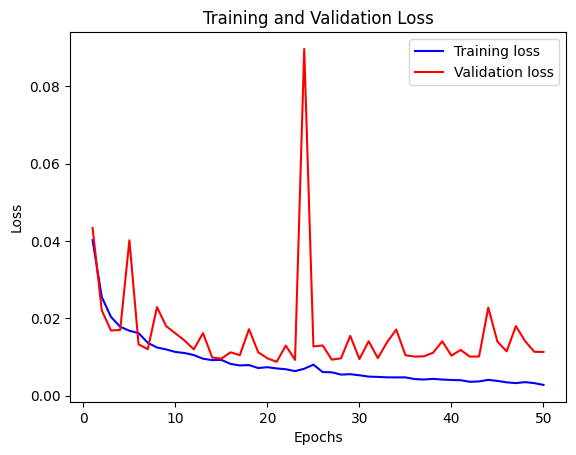
\includegraphics[width=0.75\textwidth]{indir.png}
    \caption{Training and Validation Loss Grafiği}
    \label{fig:my_pic}
\end{figure}


\subsection{(10 Puan)} \textbf{SEED=öğrenci numaranız set ettikten sonra altıncı haftada ödev olarak verdiğim gibi earlystopping'deki en iyi modeli kullanarak, Prensesi İyileştir test setinden accuracy, F1, precision ve recall değerlerini hesaplayan kodu yazın ve sonucu da aşağı yapıştırın. \%80'den fazla başarı bekliyorum test setinden. Daha düşükse başarı oranınız, nerede hata yaptığınızı bulmaya çalışın. \%90'dan fazla başarı almak mümkün (ben denedim).}

\begin{python}
from sklearn.metrics import accuracy_score, precision_score, recall_score, f1_score

# En iyi modeli kullanarak test seti uzerinde tahmin yapin
model.eval()
y_true = []
y_pred = []

for inputs, labels in test_dataloader:
    inputs = inputs.to(device)
    labels = labels.to(device)
    outputs = model(inputs)
    predictions = torch.round(outputs.squeeze())
    y_true += labels.tolist()
    y_pred += predictions.tolist()

# Test seti uzerinde olcut degerlerini hesaplayin
accuracy = accuracy_score(y_true, y_pred)
precision = precision_score(y_true, y_pred)
recall = recall_score(y_true, y_pred)
f1 = f1_score(y_true, y_pred)

# Sonuclari yazdirin
print(f"Test Accuracy: {accuracy:.4f}")
print(f"Test Precision: {precision:.4f}")
print(f"Test Recall: {recall:.4f}")
print(f"Test F1 Score: {f1:.4f}")
\end{python}

Test Accuracy: 0.9521
Test Precision: 0.9730
Test Recall: 0.9304
Test F1 Score: 0.9513

\subsection{(5 Puan)} \textbf{Tüm kodların CPU'da çalışması ne kadar sürüyor hesaplayın. Sonra to device yöntemini kullanarak modeli ve verileri GPU'ya atıp kodu bir de böyle çalıştırın ve ne kadar sürdüğünü hesaplayın. Süreleri aşağıdaki tabloya koyun. GPU için Google Colab ya da Kaggle'ı kullanabilirsiniz, iki ortam da her hafta saatlerce GPU hakkı veriyor.}

\begin{table}[ht!]
    \centering
    \caption{Çalıştırma süresi karşılaştırması}
    \begin{tabular}{c|c}
        Ortam & Süre (saniye) \\\hline
        CPU &  0:00:12.622336 \\
        GPU &  0:00:11.142654\\
    \end{tabular}
    \label{tab:my_table}
\end{table}

\subsection{(3 Puan)} \textbf{Modelin eğitim setine overfit etmesi için elinizden geldiği kadar kodu gereken şekilde değiştirin, validasyon loss'unun açıkça yükselmeye başladığı, training ve validation loss'ları içeren figürü aşağı koyun ve overfit için yaptığınız değişiklikleri aşağı yazın. Overfit, tam bir çanak gibi olmalı ve yükselmeli. Ona göre parametrelerle oynayın.}

Cevaplar buraya

% Figür aşağı
\begin{comment}
\begin{figure}[ht!]
    \centering
    \includegraphics[width=0.75\textwidth]{mypicturehere.png}
    \caption{Buraya açıklama yazın}
    \label{fig:my_pic}
\end{figure}
\end{comment}

\subsection{(2 Puan)} \textbf{Beşinci soruya ait tüm kodların ve cevapların olduğu jupyter notebook'un Github linkini aşağıdaki url'e koyun.}

\url{https://github.com/yorumusb/Yapay-Sinir-Aglari/blob/main/Soru%205.ipynb}

\section{(Toplam 10 Puan)} \textbf{Bir önceki sorudaki Prensesi İyileştir problemindeki yapay sinir ağınıza seçtiğiniz herhangi iki farklı regülarizasyon yöntemi ekleyin ve aşağıdaki soruları cevaplayın.} 

\subsection{(2 puan)} \textbf{Kodlarda regülarizasyon eklediğiniz kısımları aşağı koyun:} 

\begin{python}
import tensorflow as tf

# Model tanimi
model = tf.keras.models.Sequential([
  tf.keras.layers.Dense(64, activation='relu', input_shape=(100,), 
                        kernel_regularizer=tf.keras.regularizers.l1_l2(l1=0.01, l2=0.01)),
  tf.keras.layers.Dense(64, activation='relu', 
                        kernel_regularizer=tf.keras.regularizers.l1_l2(l1=0.01, l2=0.01)),
  tf.keras.layers.Dense(10, activation='softmax')
])

# L1 ve L2 regularizasyonu
l1_l2 = tf.keras.regularizers.l1_l2(l1=0.01, l2=0.01)

# Model tanimi
model = tf.keras.models.Sequential([
  tf.keras.layers.Dense(64, activation='relu', input_shape=(100,), kernel_regularizer=l1_l2),
  tf.keras.layers.Dense(64, activation='relu', kernel_regularizer=l1_l2),
  tf.keras.layers.Dense(10, activation='softmax')
])

\end{python}

\subsection{(2 puan)} \textbf{Test setinden yeni accuracy, F1, precision ve recall değerlerini hesaplayıp aşağı koyun:}

Sonuçlar buraya.

\subsection{(5 puan)} \textbf{Regülarizasyon yöntemi seçimlerinizin sebeplerini ve sonuçlara etkisini yorumlayın:}

Regülarizasyon yöntemlerinin seçimi, veri setinin boyutu, modelin karmaşıklığı, regülarizasyonun şiddeti ve diğer faktörlere bağlıdır.

L1 regülarizasyonu, ağırlık matrisindeki bazı ağırlıkların sıfır olduğu bir sparsity etkisi oluşturarak gereksiz özelliklerin çıkarılmasına yardımcı olabilir. Bu, veri setindeki gürültüyü azaltabilir ve modelin daha genelleştirilebilir hale gelmesine yardımcı olabilir. Ancak, L1 regülarizasyonu, ağırlıkların bir kısmını tamamen sıfır hale getirdiği için bazı bilgilerin kaybolmasına neden olabilir.

L2 regülarizasyonu, ağırlık matrisinin tüm elemanları üzerinde küçük bir etkiye sahip olur ve tüm ağırlık matrisini küçültür. Bu, modelin overfitting eğilimini azaltır ve daha iyi genelleştirme performansı sağlayabilir. Ayrıca, L2 regülarizasyonu, modelin hiperparametrelerinin daha iyi optimize edilmesine yardımcı olabilir.

\subsection{(1 puan)} \textbf{Sonucun github linkini  aşağıya koyun:}

\url{www.benimgithublinkim2.com}

\end{document}